


\documentclass[ChapterTOCs,krantz1]{krantz}
\usepackage{graphicx, color}
%% maxwidth is the original width if it is less than linewidth
%% otherwise use linewidth (to make sure the graphics do not exceed the margin)
\makeatletter
\def\maxwidth{ %
  \ifdim\Gin@nat@width>\linewidth
    \linewidth
  \else
    \Gin@nat@width
  \fi
}
\makeatother

\IfFileExists{upquote.sty}{\usepackage{upquote}}{}
\definecolor{fgcolor}{rgb}{0.2, 0.2, 0.2}
\newcommand{\hlnumber}[1]{\textcolor[rgb]{0,0,0}{#1}}%
\newcommand{\hlfunctioncall}[1]{\textcolor[rgb]{0.501960784313725,0,0.329411764705882}{\textbf{#1}}}%
\newcommand{\hlstring}[1]{\textcolor[rgb]{0.6,0.6,1}{#1}}%
\newcommand{\hlkeyword}[1]{\textcolor[rgb]{0,0,0}{\textbf{#1}}}%
\newcommand{\hlargument}[1]{\textcolor[rgb]{0.690196078431373,0.250980392156863,0.0196078431372549}{#1}}%
\newcommand{\hlcomment}[1]{\textcolor[rgb]{0.180392156862745,0.6,0.341176470588235}{#1}}%
\newcommand{\hlroxygencomment}[1]{\textcolor[rgb]{0.43921568627451,0.47843137254902,0.701960784313725}{#1}}%
\newcommand{\hlformalargs}[1]{\textcolor[rgb]{0.690196078431373,0.250980392156863,0.0196078431372549}{#1}}%
\newcommand{\hleqformalargs}[1]{\textcolor[rgb]{0.690196078431373,0.250980392156863,0.0196078431372549}{#1}}%
\newcommand{\hlassignement}[1]{\textcolor[rgb]{0,0,0}{\textbf{#1}}}%
\newcommand{\hlpackage}[1]{\textcolor[rgb]{0.588235294117647,0.709803921568627,0.145098039215686}{#1}}%
\newcommand{\hlslot}[1]{\textit{#1}}%
\newcommand{\hlsymbol}[1]{\textcolor[rgb]{0,0,0}{#1}}%
\newcommand{\hlprompt}[1]{\textcolor[rgb]{0.2,0.2,0.2}{#1}}%

\usepackage{framed}
\makeatletter
\newenvironment{kframe}{%
 \def\at@end@of@kframe{}%
 \ifinner\ifhmode%
  \def\at@end@of@kframe{\end{minipage}}%
  \begin{minipage}{\columnwidth}%
 \fi\fi%
 \def\FrameCommand##1{\hskip\@totalleftmargin \hskip-\fboxsep
 \colorbox{shadecolor}{##1}\hskip-\fboxsep
     % There is no \\@totalrightmargin, so:
     \hskip-\linewidth \hskip-\@totalleftmargin \hskip\columnwidth}%
 \MakeFramed {\advance\hsize-\width
   \@totalleftmargin\z@ \linewidth\hsize
   \@setminipage}}%
 {\par\unskip\endMakeFramed%
 \at@end@of@kframe}
\makeatother

\definecolor{shadecolor}{rgb}{.97, .97, .97}
\definecolor{messagecolor}{rgb}{0, 0, 0}
\definecolor{warningcolor}{rgb}{1, 0, 1}
\definecolor{errorcolor}{rgb}{1, 0, 0}
\newenvironment{knitrout}{}{} % an empty environment to be redefined in TeX

\usepackage{alltt}
\newcommand{\SweaveOpts}[1]{}  % do not interfere with LaTeX
\newcommand{\SweaveInput}[1]{} % because they are not real TeX commands
\newcommand{\Sexpr}[1]{}       % will only be parsed by R


\usepackage{amssymb}
\usepackage{amsmath}
\usepackage{graphicx}
\usepackage{subfigure}
%\usepackage{epsfig}
\usepackage{makeidx}
%\usepackage{showidx}
\usepackage{multicol}
\frenchspacing
\tolerance=5000

\usepackage{dcolumn}
\usepackage{booktabs}
\usepackage{url}
\usepackage{todonotes}
\usepackage{tikz}




\makeatletter


\makeatother

\makeindex



\begin{document}
% Chapter Chapter 3 For Reproducible Research in R and RStudio
% Christopher Gandrud
% Created: 16/07/2012 05:45:03 pm CEST
% Updated: 22 August 2012




\chapter{Getting Started with R and RStudio}

If you have rarely or never used R before the first two sections of this chapter give you enough information that you should be able to get started and understand the code I use in this book. For more details about R please refer to the related resources I mentioned in chapter \ref{WhatNot}. Experienced R users might want to skip the first two sections of the chapter. This chapter also gives a brief overview of RStudio. It highlights the key features of main RStudio panel (what appears when you open RStudio) and some of its key features for reproducible research.

\section{Installing R and RStudio}

R and RStudio are open source programs and can be easily downloaded for free. Both are available for Windows, Mac, and Unix. They should run well on most modern computers. 

You should install R before installing RStudio. You can down load the programs from the following websites:

\begin{itemize}
    \item {\bf{R}}: \url{http://www.r-project.org/},
    \item {\bf{RStudio}}: \url{http://rstudio.org/download/}.
\end{itemize}

\noindent The download webpages for these programs have comprehensive information on how to install them, so please refer to those pages for more information.

\paragraph{Installing markup languages}

If you are planning on creating \LaTeX documents you need to install a \index{\LaTeX distribution}. They are also open source and available for Windows, Mac, and Unix. They can be found at: \url{http://www.latex-project.org/ftp.html}. Please refer to that site for more installation information.

If you want to create markdown documents you will need to install the the \index{{\emph{markdown}} package} in R. You can do this the same way that you install any package in R, with the {\tt{install.packages}} command.\footnote{The exact command is: {\tt{install.packages("markdown")}}.} 

\section{Using R: the basics}

\subsection{Objects \& Assignment}

\subsection{Component Selection}

\subsection{Functions, Commands, and Arguments}

\section{Using RStudio}

When you first open RStudio you should get a something that looks like Figure \ref{BlankMain}. In this figure you see three panels. The large one on the left is the {\emph{Console}}. This pane functions exactly the same as 

\begin{figure}[t]
    \caption{RStudio Startup Panel}
    \label{BlankMain}

    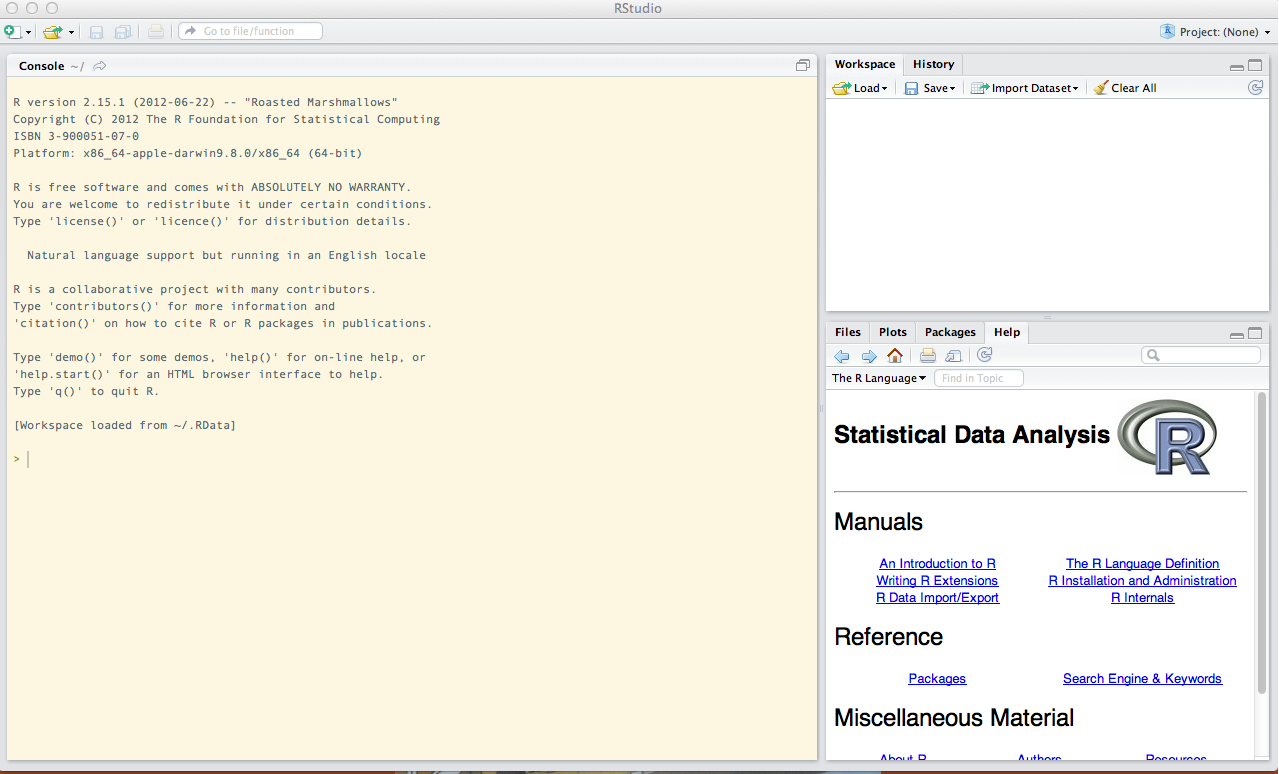
\includegraphics[width = \textwidth]{/git_repositories/Rep-Res-Book/Source/Children/Chapter3/images3/BlankMainPanel.png}
\end{figure}


\section{Tips}

Here are a few tips that make using R and RStudio a little easier.

\paragraph{Autocomplete}

In R and RStudio you do not have to type out every command, argument, or object name. On Mac and Unix based versions of R after you start typing a command or object name you can hit the ``tab" key to automatically complete what you are typing. The \index{autocomplete} function is particularly good in RStudio. Not only does it give you a list of words to choose from, but it also shows you an abbreviated version of the help file for commands and arguments.

\end{document}
